%%%%%%%%%%%%%%%%%%%%%%%%%%%%%%%%%%%%%%%%%%%%%
% PROCESAMIENTO DIGITAL DE SEÑALES DE AUDIO
% MAESTRÍA EN INGENIERÍA ELÉCTRICA, UDELAR
% SEGUNDO SEMESTRE 2016
%%%%%%%%%%%%%%%%%%%%%%%%%%%%%%%%%%%%%%%%%%%%%

%----------------------------------------------------------------------------------------
%	PACKAGES AND DOCUMENT CONFIGURATIONS
%----------------------------------------------------------------------------------------

\documentclass{article}

\usepackage[version=3]{mhchem} % Package for chemical equation typesetting
\usepackage{siunitx} % Provides the \SI{}{} and \si{} command for typesetting SI units

\usepackage[spanish]{babel}
\selectlanguage{spanish}
\usepackage[utf8]{inputenc}
\usepackage{graphicx} % Required for the inclusion of images
\usepackage{natbib} % Required to change bibliography style to APA
\usepackage{amsmath} % Required for some math elements 

\usepackage{float}

\usepackage{geometry}
 \geometry{
 a4paper,
 total={170mm,257mm},
 left=20mm,
 top=20mm,
 }

\usepackage{listings}
\usepackage{color} %red, green, blue, yellow, cyan, magenta, black, white
\definecolor{mygreen}{RGB}{28,172,0} % color values Red, Green, Blue
\definecolor{mylilas}{RGB}{170,55,241}

\lstset{language=Matlab,%
    %basicstyle=\color{red},
    breaklines=true,%
    morekeywords={matlab2tikz},
    keywordstyle=\color{blue},%
    morekeywords=[2]{1}, keywordstyle=[2]{\color{black}},
    identifierstyle=\color{black},%
    stringstyle=\color{mylilas},
    commentstyle=\color{mygreen},%
    showstringspaces=false,%without this there will be a symbol in the places where there is a space
    numbers=left,%
    numberstyle={\tiny \color{black}},% size of the numbers
    numbersep=9pt, % this defines how far the numbers are from the text
    emph=[1]{for,end,break},emphstyle=[1]\color{red}, %some words to emphasise
    %emph=[2]{word1,word2}, emphstyle=[2]{style},    
}

\setlength\parindent{0pt} % Removes all indentation from paragraphs

\renewcommand{\labelenumi}{\alph{enumi}.} % Make numbering in the enumerate environment by letter rather than number (e.g. section 6)


%----------------------------------------------------------------------------------------
%	DOCUMENT INFORMATION
%----------------------------------------------------------------------------------------

\title{\textbf{Informe Final - Proyecto 2016}\\\large \textsc{Procesamiento digital de señales de audio}\\
 \textsc{Maestría en Ingeniería Eléctrica} del \textit{Instituto de Ingeniería Eléctrica, Facultad de Ingeniería, Universidad de la República.}}

\author{\textit{Juan Braga}}
\date{\today}

\begin{document}

\maketitle 

%----------------------------------------------------------------------------------------
%	EJERCICIO 1
%----------------------------------------------------------------------------------------

\section*{Extracción de embocadura en Aliento/Arrugas: Introducción}
En Aliento/Arrugas de Marcelo Toledo se utiliza como recurso expresivo tres tipos de embocadura para ejecución de la flauta. Se diferencian por el ángulo que forma el flujo de aire frente al filo de la embocadura. Se enlista a continuación los nombres de cada una, manteniendo su denominación en Inglés (idioma utilizado en la partitura de la obra). Además en la Figura \ref{fig:embocaduras} se observa su notación en la partitura de Aliento/Arrugas.

\begin{itemize}
  \item \textit{Normal Embrochure}: Embocadura clásica de la flauta, donde el el flujo de aire frente al filo de la embocadura genera la exitación tonal. 
  \item \textit{Blow Hole Covered}: El flujo de aire ingresa directo al tubo de la flauta, sin generar turbulencia contra el filo de la embocadura. 
  \item \textit{Breathy Embrochure}: Caso intermedio entre las otras dos embocaduras. 
\end{itemize}
\medskip

\begin{figure}[H]
\begin{center}
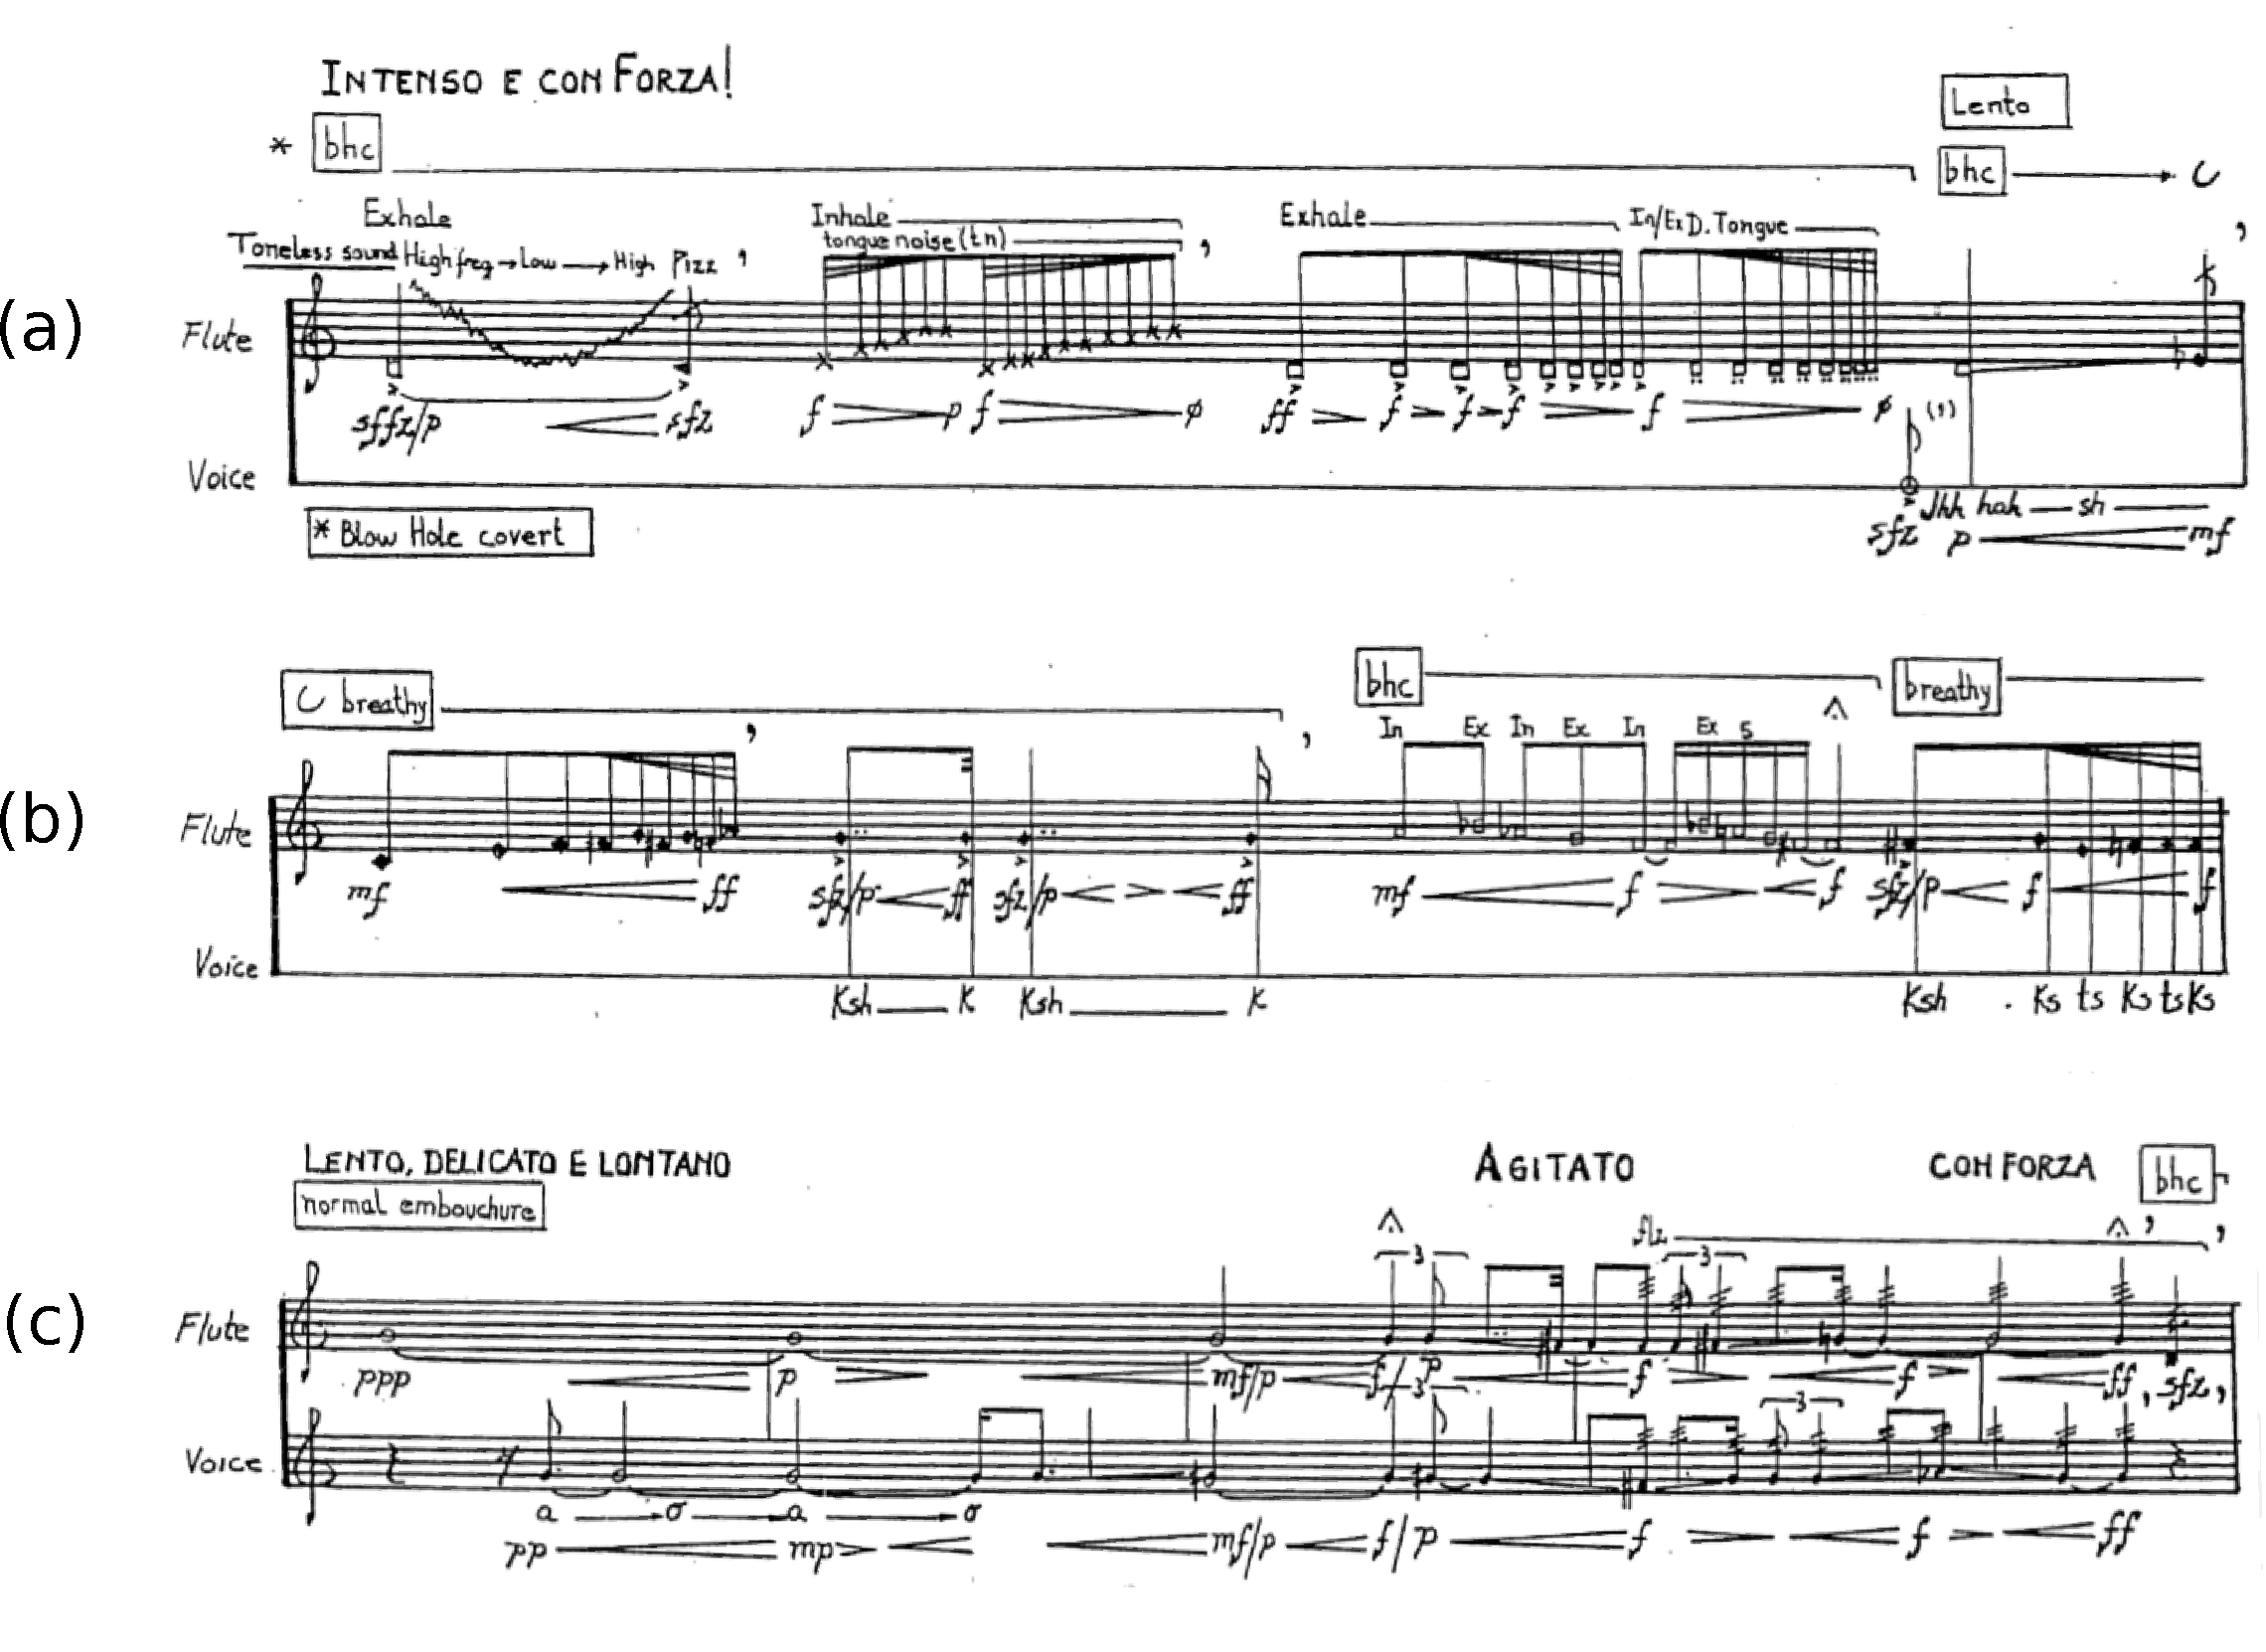
\includegraphics[width=0.9\textwidth]{embocaduras} 
\caption{Notación de las embocaduras se observa en la parte superior de los sistemas. (a) \textit{Blow Hole Covered}. (b) \textit{Breathy Embrochure}. (c) \textit{Normal Embrochure}. Fragmentos extraídos de la partitura de Aliento/Arrugas.}
\label{fig:embocaduras}
\end{center}
\end{figure}

\section*{Definición del Problema}
Se propone la extracción automática del tipo de embocadura a través del análisis computacional de grabaciones de la obra. 

\section*{Datos}
Se cuenta con 5 grabaciones de diferentes intérpretes de la obra Aliento/Arrugas. Los intérpretes son: Pablo Somma, Emma Resmini, Claire Chase, Juan Pablo Quinteros y Ulla Suokko. Los archivos de audio se etiquetaron utilizando el software \textit{Sonic Visualizer} dividiendo los fragmentos de audio en 5 clases:

\begin{itemize} 
  \item Silencio.
  \item Silencio con respiración del intérprete. 
  \item Sonido generado con \textit{Blow Hole Covered}.
  \item Sonido generado con \textit{Breathy Embrochure}.
  \item Sonido generado con \textit{Normal Embrochure}.
\end{itemize}

Para el presente informe se trabaja con las tres últimas clases de la lista anterior. 

\section{Análisis de la naturaleza sonora del problema}

Se cree que se puede separar con características que describan el nivel de peridicidad de la señal. 
Primer experimento: con Voicing y ZCR \citep[Chapter~4]{rabiner1978digital}
El compositor 
Color
Material sonoro
Embocadura

\section{Estrategia de resolución}

Se trata de resolver el problema con un enfoque de reconocimiento de patrones. Se procesa el audio como un \textit{Bag of Frames} a partir del computo de características. Se utilizan tres algoritmos clásicos de clasificación para evaluación del desempeño de las características en la extracción automática de embocadura a partir de las muestras de audio.

   
\subsection{Experimentos}

Se evalúa el desempeño de características de diversa naturaleza en la extracción del tipo de embocadura. Todos los experimentos se realizan con \textit{5-fold cross validation} donde los folds son las diferentes interpretaciones de la pieza musical. De esta forma se asegura que frames provenientes de la misma grabación no sean usados para train y test en un mismo experimento.
\medskip

Se utilizan tres clasificadores distintos para minimizar el bías que pueda existir entre los datos y un algoritmo en particular. Se trabaja con los algoritmos: \textit{Random Forest (trees=10)}, \textit{Support Vector Machine (kernel lineal)} y \textit{K-Nearest Neighbors (k=10)}. En todos los casos se utilizan los parámetros por defecto ya que no es objetivo de este trabajo encontrar los valores óptimos de clasificación. La implementación se realiza mediante el módulo de \textit{Python} llamado \textit{Scikit Learn} \citep{pedregosa2011scikit}. En todos los casos los datos son preprocesados de manera de centrar en cero y escalar la varianza a uno, previo al clasificador.
\medskip

\subsection{Extración de características}
Se enlistan a continuación las características que se evalúan la extracción automática de embocadura. Además se describe brevemente sus principales características.

\begin{itemize} 
  \item Características Clásicas
  \item MFCC 
  \item LPC
  \item Spectral Contrast \citep{jiang2002music}
\end{itemize}

\subsection{Resultados}
Accuracy

Confusión de MFCC:

\subsection{Experimentos 2}
MFCC es un fierro pero apriori no tiene porque utilizar la información de periodicidad propiamente dicha. Parámetro relevante en la separación de estos tres tipos de embocadura. Se agrega voicing tipo yin \cite{de2002yin}



Se identifica nuevamente el problema en la separación

Comparar confusión entre 2x2 y 3x3 en la separación de BHC y BREATHY

Discusión de agregar voicing, ver como mejora la matriz de confusión 

\subsubsection{}


\section{Trabajo a futuro}

\begin{itemize} 
  \item Segmentación de audio, umbralizando los silencios y las respiraciones 
  \item Salir del bag of frames, para utilizar la redundancia temporal
\end{itemize}
%----------------------------------------------------------------------------------------
%	BIBLIOGRAPHY
%----------------------------------------------------------------------------------------


\newpage
\bibliographystyle{apalike}
\bibliography{biblio}


%----------------------------------------------------------------------------------------
\end{document}


